\documentclass[12pt]{article}
\usepackage{latexblog}

% ============================================================
% Blog Metadata
% ============================================================
\blogtitle{OAuth 2.0的一些问题}
\blogdate{2020-12-01}
\blogtags{刨根问底, OAuth, 协议}
\bloglang{zh}
\blogsummary{}

\begin{document}
\makeblogtitle

OAuth2或者OIDC是一个比较复杂的问题，但是很多人用的时候都是一知半解，所以出现一些不正确或者不建议的做法。

\section{应用场景}\label{ux5e94ux7528ux573aux666f}

一个是在什么情况下应该使用OAuth/OIDC的问题。

\begin{figure}
\centering
\pandocbounded{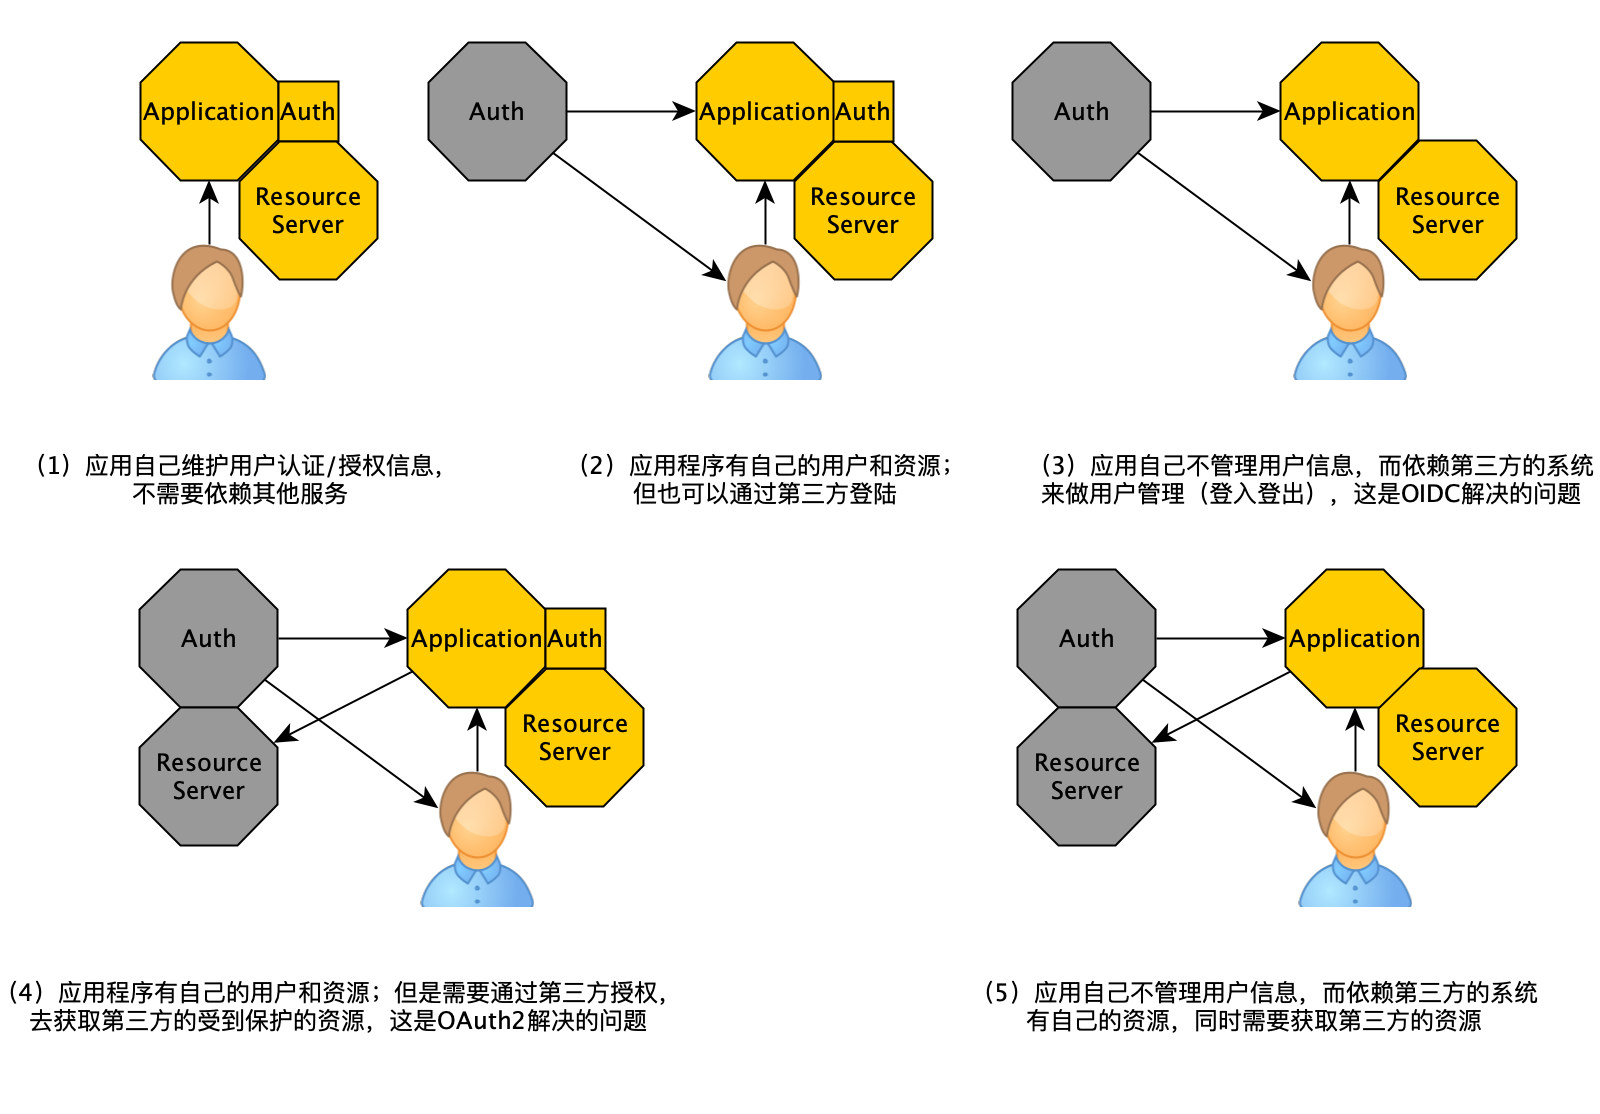
\includegraphics[keepaspectratio,alt={Cases}]{images/OAuth_OIDC_cases.png}}
\caption{Cases}
\end{figure}

\begin{itemize}
\tightlist
\item
  第一种是应用自己完成认证授权的流程，通常的做法是通过用户名和密码登录认证；然后通过规则来判断用户是否有权限进行某些操作；这种跟OAuth没有半毛线关系
\item
  第二种是，在第一种的基础上，应用也希望能够通过第三方登录（但同时自己也有一套用户机制），也就是典型的``social login''，那么应该考虑使用OIDC
\item
  第三种是应用自己没有用户体系，需要借助第三方来进行认证，但应用自己管理资源。这种情况下也需要用OIDC来进行登陆认证，跟第二种没有实质的区别
\item
  第四种是，在第一种的基础上，假设应用还需要访问一些其他的受保护的资源，比如你写博客的时候想用QQ空间的照片。那么应该通过OAuth2来获取对这个资源的访问权限即可
\item
  第五种情况，应用通过第三方进行认证，有自己的资源；但同时也需要访问其他受保护的资源。这里认证肯定还是需要通过OIDC来实现；访问受保护的资源使用OAuth2即可。对于用户自己的资源，可以根据自己的需要进行管理，而不需要通过什么access\_token。
\end{itemize}

这里有一个很大的误区就是，认为凡是授权都需要OAuth2，譬如第五种情况，的确我们通过OIDC完成认证体系；那么问题是，假设我访问自己的resource，是否需要走一遍OAuth2的流程？试想我们这么做，那么可能会变成这样：

\begin{itemize}
\tightlist
\item
  用户通过QQ登陆到你开发的一个博客网站，很开心，想自己去写博客什么的
\item
  用户现在想去看自己的博客，而你需要得到一个access\_token，所以会弹出一个框告诉用户，你要访问你的博客，是否允许\ldots{} 这不是很扯淡么。如果我认证之后每次都还需要这样做一次，那有什么意义存在呢？
\item
  好吧，假设说你用一个client credential的流程，这样应用自己可以去请求一个access\_token了，不需要用户参与。这样是否可行呢？
\end{itemize}

如果client app跟resource server是同一个应用，那么这样相当于我自己去拿一个token，然后我自己验证这个token，然后知道我是否有权限。且不论效率问题，唯一可能的场景就是必须要通过OAuth Server来获取用户的权限，但通常这些规则也必须要进行设置（那为什么要到OAuth中设置？这样通常代价更高）。

如果client app跟resource server不是一个应用，这样做倒是可以实现一个统一的权限管理机制，不过，唯一的问题就是性能问题。

\section{Token相关}\label{tokenux76f8ux5173}

\subsection{Token的存储}\label{tokenux7684ux5b58ux50a8}

\subsubsection{Web APP}\label{web-app}

\begin{itemize}
\tightlist
\item
  如果应用有服务端，那么token存储在服务端。浏览器通过session跟服务器交互
\item
  如果没有服务端，那么id\_token和access\_token应该存储在浏览器的内存中
\item
  如果不得不存储在浏览器，那么可以通过加密之后存储在session cookie中
\end{itemize}

\begin{figure}
\centering
\pandocbounded{\includegraphics[keepaspectratio,alt={Next.js}]{https://images.ctfassets.net/cdy7uua7fh8z/6a4aA0TH8PJQpvhkLaGSIp/e38aae00318515f2a0efa0dfce24dca2/in-memory-token-storage.png}}
\caption{Next.js}
\end{figure}

\subsubsection{Native/Mobile app}\label{nativemobile-app}

可以存储在OS提供的安全存储中，例如：

\begin{itemize}
\tightlist
\item
  安卓中使用KeyStore
\item
  iOS中使用KeyChain
\end{itemize}

\subsubsection{SPA单页应用}\label{spaux5355ux9875ux5e94ux7528}

跟Web APP一样，如果SPA有对应的后端支持，token应该存储在SPA的后端，但是SPA需要通过某种机制去获取这个token；如果没有对应的后端，那么只能存储在内存中。

\subsubsection{id\_token可以当access\_token使用么}\label{id_tokenux53efux4ee5ux5f53access_tokenux4f7fux7528ux4e48}

id\_token是由授权服务器颁发给client的，比如请求一个id\_token的：

\begin{verbatim}
https://authorization-server.com/authorize?
  response_type=code
  &client_id=egHuu4oJxgOLeBzPAQ9sXg4i
  &redirect_uri=https://www.oauth.com/playground/oidc.html
  &scope=openid+profile+email+photos
  &state=sRROJ_iPTam39Dc7
  &nonce=eFRvo_n5ecyYU_Sv
\end{verbatim}

最后得到的id\_token是这样的：

\begin{Shaded}
\begin{Highlighting}[]
\FunctionTok{\{}
  \DataTypeTok{"sub"}\FunctionTok{:} \StringTok{"concerned{-}caracal@example.com"}\FunctionTok{,}
  \DataTypeTok{"name"}\FunctionTok{:} \StringTok{"Concerned Caracal"}\FunctionTok{,}
  \DataTypeTok{"email"}\FunctionTok{:} \StringTok{"concerned{-}caracal@example.com"}\FunctionTok{,}
  \DataTypeTok{"iss"}\FunctionTok{:} \StringTok{"https://pk{-}demo.okta.com/oauth2/default"}\FunctionTok{,}
  \DataTypeTok{"aud"}\FunctionTok{:} \StringTok{"egHuu4oJxgOLeBzPAQ9sXg4i"}\FunctionTok{,}
  \DataTypeTok{"iat"}\FunctionTok{:} \DecValTok{1600674514}\FunctionTok{,}
  \DataTypeTok{"exp"}\FunctionTok{:} \DecValTok{1603266514}\FunctionTok{,}
  \DataTypeTok{"amr"}\FunctionTok{:} \OtherTok{[}
    \StringTok{"pwd"}
  \OtherTok{]}
\FunctionTok{\}}
\end{Highlighting}
\end{Shaded}

这里\texttt{aud}即client的id，是可以被client所信任的。而id\_token不是设计给resource server使用的，所以显然不能使用id\_token代替access\_token。

References:

\begin{itemize}
\tightlist
\item
  \href{https://auth0.com/docs/applications}{Applications in Auth0}
\item
  \href{https://alexbilbie.com/guide-to-oauth-2-grants/}{A Guide To OAuth 2.0 Grants}
\item
  \href{https://openid.net/connect/faq/}{OpenID Connect FAQ and Q\&As}
\item
  \href{https://auth0.com/docs/authorization/authentication-and-authorization}{Authentication and Authorization}
\item
  \href{https://stackoverflow.com/questions/48544500/oauth-and-authentication}{OAuth and authentication}
\item
  \href{https://www.scottbrady91.com/OAuth/OAuth-is-Not-Authentication}{OAuth is Not Authentication}
\item
  \href{https://openid.net/specs/openid-connect-core-1_0.html}{OpenID Connect Core 1.0 incorporating errata set 1}
\end{itemize}


\end{document}
